\section{Matrices, maps and decompositions}
Hopefully these pictures will reinforce basic concepts between matrices, their maps and their decomposition.

The three basic types of problems we considered are listed below. We will see the matrix \svdl, the transpose matrix \svdl, and the pseudoinverse expressed in terms of the decomposition matrices.
\begin{enumerate}
%
\item full rank: no rank deficits for either row or column space
\subitem no null space vectors in either $\X{}$ or $\Y{}$
\subitem both maps, $\A{}$ and $\A{T}$, are reversible
\subitem the pseudoinverse is the standard inverse
%
\item full row rank but column rank deficient
\subitem null space vectors (gray) in  $\X{}$
\subitem only the $\A{T}$ map is reversible
\subitem the pseudoinverse is a right inverse
%
\item both row and column rank deficient 
\subitem null space vectors (gray) in both $\X{}$ and $\Y{}$
\subitem neither map, $\A{}$ or $\A{T}$, is reversible
\subitem the pseudoinverse is neither a left nor a right inverse
%
\end{enumerate}

\clearpage

%%
%% 2 x 2
%%
\begin{center}
\includegraphics[]{pdf/post_mortemII/C222}\\
\end{center}

\begin{table}[htdp]
\begin{center}
\begin{tabular}{cc}
  $\A{}x=y$ & $\A{T}y=x$\\
$\mat{rr}{1&2\\-1&2}\mat{c}{x_{1}\\x_{2}} = \mat{c}{y_{1}\\y_{2}}$ &
$\mat{rr}{1&-1\\2&2}\mat{c}{x_{1}\\x_{2}} = \mat{c}{y_{1}\\y_{2}}$ \\
\ \\
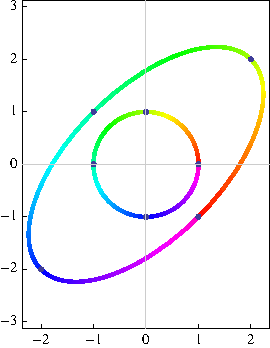
\includegraphics[ width = 2.15in ]{pdf/post_mortemII/2_2_2} &
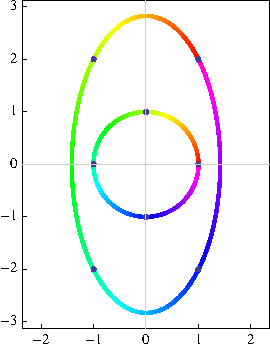
\includegraphics[ width = 2.15in ]{pdf/post_mortemII/2_2_2_t} \\
%%
\ \\
\end{tabular}
\end{center}
\label{tab:proj:a}
\caption[Case 1 - full rank]{Case 1 - full rank: no rank deficits for either row or column space.}
\end{table}%

\begin{equation*}
  \begin{array}{lcccrcr}
     \A{} &=& \svd{T} &=& \stwo \mat{rr}{1&1\\1&-1} & 
     \sqrt{2} \mat{cc}{2&0\\0&1} &
     \ktwo\\[5pt]
     \A{T} &=& \svdt{T} &=& \ktwo & \sqrt{2} \mat{cc}{2&0\\0&1} & \stwo \mat{rr}{1&1\\1&-1}\\[5pt]
     \Ap &=& \mpgi{T} &=& \ktwo & \stwo \mat{cc}{\rtwo&0\\0&1} & \stwo \mat{rr}{1&1\\1&-1}
  \end{array}
\end{equation*}

\clearpage
%%
%% 2 x 3
%%
\begin{center}
\includegraphics[  ]{pdf/general/C232}
\end{center}
\begin{table}[htdp]
\begin{center}
\begin{tabular}{cc}
  $\A{}x=y$ & $\A{T}y=x$\\
$\mat{ccc}{0&3&0\\1&1&2}\mat{c}{x_{1}\\x_{2}\\x_{3}} = \mat{c}{y_{1}\\y_{2}}$ &
$\mat{cc}{0&1\\3&1\\0&2}\mat{c}{y_{1}\\y_{2}} = \mat{c}{x_{1}\\x_{2}\\x_{3}}$ \\
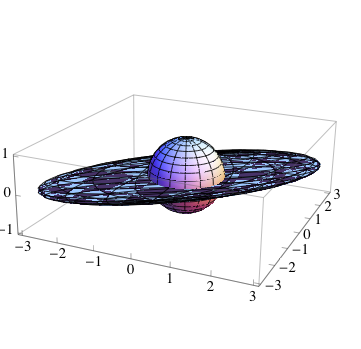
\includegraphics[ width = 2.5in ]{pdf/post_mortemII/3_2_2.png} &
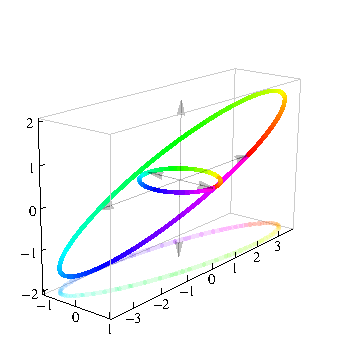
\includegraphics[ width = 2.5in ]{pdf/post_mortemII/3_2_2_t} \\
%%
\end{tabular}
\end{center}
\label{tab:proj:b}
\caption[Case 2 - full row rank, column rank deficient]{Case 2 - full row rank but column rank deficient.}
\end{table}
%%%
{\tiny
\begin{equation*}
  \begin{array}{lllll}
     \svda{T} = &  \stwo
  \mat{rr}{1 & -1\\1 & 1}
  \ 
  \mat{cc|c}
  {\sqrt{15} & 0 & 0 \\
  0 & \sqrt{3}  & 0}
  \ 
  \mat{ crr }
 {\frac{1}{\sqrt{30}} & \frac{5}{\sqrt{30}} & \frac{2}{\sqrt{30}}\\
  \ssix & \frac{-1}{\sqrt{6}} & \frac{2}{\sqrt{6}} \\
  \rowcolor{ltgray}
  \frac{-2}{\sqrt{5}} & 0 & \sfive}\\
  \end{array}
\end{equation*}
%%
\begin{equation*}
  \begin{array}{lllll}
     \A{T} &= \svdt{T} = &
     \mat{rr>{\columncolor{ltgray}}r}
     { \frac{1}{\sqrt{30}} & \ssix               & \frac{-2}{\sqrt{5}} \\
       \frac{5}{\sqrt{30}} & \frac{-1}{\sqrt{6}} & 0 \\
       \frac{2}{\sqrt{30}} & \frac{2}{\sqrt{6}}  & \frac{1}{\sqrt{5}} }
     & \mat{cc}{\sqrt{15}&0\\0&\sqrt{3}\\\hline0&0} & \stwo \mat{rr}{1&1\\-1&1}\\[5pt]
  %%
     \mpgia{T} = &
     \mat{rr>{\columncolor{ltgray}}r}
     { \frac{1}{\sqrt{30}} & \ssix            & \frac{-2}{\sqrt{5}} \\
       \frac{5}{\sqrt{30}} & \frac{-1}{\sqrt{6}} & 0 \\
       \frac{2}{\sqrt{30}} & \frac{2}{\sqrt{6}}  & \frac{1}{\sqrt{5}} }
     & \mat{cc}{\frac{1}{\sqrt{15}}&0\\0&\frac{1}{\sqrt{3}}\\[5pt]\hline0&0}
     & \stwo \mat{rr}{1&1\\-1&1}
  \end{array}
\end{equation*}
}
\clearpage
%%
%% 3 x 2
%%
\begin{center}
\includegraphics[  ]{pdf/simple/C321}\\
\end{center}
\begin{table}[htdp]
\begin{center}
\begin{tabular}{cc}
  $\A{}x=y$ & $\A{T}y=x$\\
$\Aexample \mat{c}{x_{1}\\x_{2}} = \mat{c}{y_{1}\\y_{2}\\y_{3}}$ &
$\Atexample\mat{c}{x_{1}\\x_{2}\\x_{3}} = \mat{c}{y_{1}\\y_{2}}$ \\
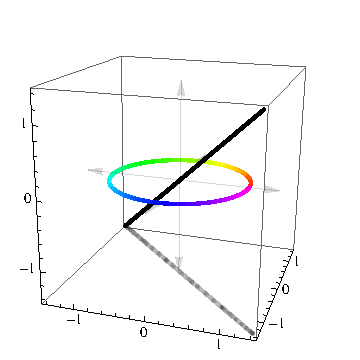
\includegraphics[ width = 2.5in ]{pdf/post_mortemII/3_2_1_a} &
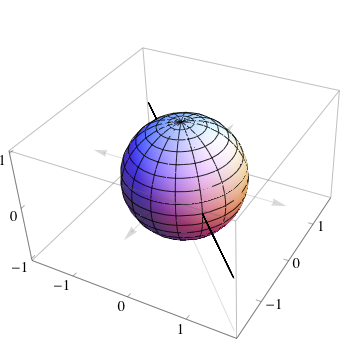
\includegraphics[ width = 2.5in ]{pdf/post_mortemII/3_2_1_t_a} \\
%%
\end{tabular}
\end{center}
\label{tab:proj:c}
\caption[Case 3 - row and column rank deficient]{Case 3 - both row and column rank deficient.}
\end{table}

{\tiny{
\begin{equation*}
  \begin{array}{lllll}
     \A{} &= \svd{T} = &\Yshade \Sigmaexampleb \Xtshade\\
  \end{array}
\end{equation*}
\begin{equation*}
  \begin{array}{lllll}
     \A{T} &= \svdt{T} = & \Xshade & \Sigmatexamplea & \Ytshade\\[5pt]
     \mpgia{T} = & \Xshade & \Sigmainverse & \Ytshade\\
  \end{array}
\end{equation*}
}}

\clearpage
\endinput
